\begin{Ueberlieferung}% 
{\textit{L}}Konzept: LH XXXVII 5 Bl. 128-129. 1 Bog. 2\textsuperscript{o}. 4 S. zumeist einspaltig. Ein Wasserzeichen auf Bl.~129.\\%
Cc 2, Nr. 969
\end{Ueberlieferung}
%
\begin{Datierungsgruende}%
Das vorliegende Stück N.~15 %?? = 37,05_128-129
weist das gleiche Wasserzeichen auf
wie die Stücke N.~19-21 und N.~23-26. %?? = Bruchfestigkeit
Daher lässt sich auch N.~15 %?? = 37,05_128-129
auf September 1672 bis März 1673 datieren.
\end{Datierungsgruende}
%
\count\Afootins=1200
\count\Bfootins=1000
\count\Cfootins=1200
\pstartfirst%
[128~r\textsuperscript{o}]
\pend
\pstart
\centering%
De Motu gravium\protect\index{Sachverzeichnis}{grave} \edlabel{LH037,05_128r_title-01}%
naturali%
\edtext{}{{\xxref{LH037,05_128r_title-01}{LH037,05_128r_title-02}}{\lemma{naturali}\Bfootnote{%
\textit{(1)}\ Suppona %
\textit{(2)}\ Certum est %
\textit{(3)}\ Supponamus \textit{L}}}}%
\pend
\vspace{1em}
\pstart 
\noindent%
Supponamus\edlabel{LH037,05_128r_title-02} grave\protect\index{Sachverzeichnis}{grave}
\edtext{in}{\lemma{in}\Bfootnote{\textit{erg. L}}}
\edtext{quolibet puncto lineae tendentiae}{\lemma{quolibet}\Bfootnote{\textit{(1)}\ momento inter \textit{(2)}\ puncto lineae tendentiae \textit{L}\ }}
descendendum impetum\protect\index{Sachverzeichnis}{impetus} accipere \edtext{novum. \\ 
\indent Hos}{\lemma{novum}\Bfootnote{\textit{(1)}\ Eadem enim \textit{(2)}\ Cum enim caus \textit{(3)}\ Hos \textit{L}\ }} impetus\protect\index{Sachverzeichnis}{impetus} novos supponamus esse inter se aequales. Etsi enim alibi demonstraverim \edtext{eos esse minores in}{\lemma{eos}\Bfootnote{\textit{(1)}\ tanto esse minores quanto \textit{(2)}\ esse minores in \textit{L}\ }} \edtext{grave profundius seu quod jam}{\lemma{grave}\Bfootnote{\textit{(1)}\ propius accedit magis \textit{(2)}\ profundius seu quod jam \textit{L}\ }} descendit, quam in altius, quia tamen ea differentia nisi in magnis spatiis non fit sensibilis, ideo impraesentiarum, supponamus esse \setline{16}aequales.
\pend 
\pstart 
\begin{window}[0,r,\hspace{2mm}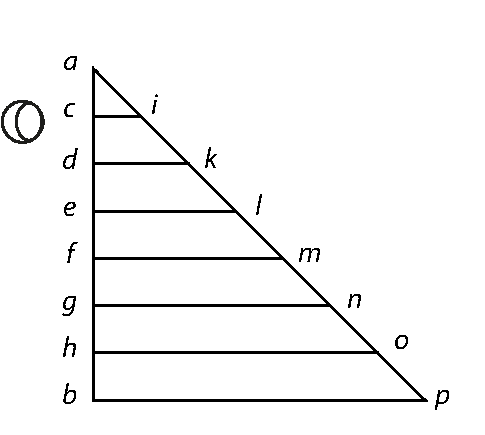
\includegraphics[%trim = -3mm -2mm 0mm 0mm, clip,
width=0.38\textwidth]
{images/lh03705_128r-d.pdf}, \hspace{25mm}{[\textit{Fig. 1}]}]
{Porro\reversemarginpar\marginnote{\scriptsize\hspace{-13mm}15}} impetus\protect\index{Sachverzeichnis}{impetus} singuli, quovis momento accepti, comparari possunt puncto.
\\
\indent Ergo summa impetuum\protect\index{Sachverzeichnis}{impetus}, in quovis momento possessorum, seu impetus\protect\index{Sachverzeichnis}{impetus} integer in quovis post primum, descensus momento exhiberi potest linea.
\\
\indent {Esto\reversemarginpar\marginnote{\scriptsize\hspace{-13mm}20}} enim linea\protect\index{Sachverzeichnis}{linea tendentiae} \edtext{tendentiae a gravi descendente percurrenda}{\lemma{20f. \hspace{1.8mm} tendentiae}\killnumber\Bfootnote{\textit{(1)}\ percursa  \textit{(2)}\ a gravi descendente percurrenda \textit{L}}} \edtext{$ab$ quae dividi intelligatur, in puncta quotlibet}{\lemma{21f. \hspace{1.8mm} $ab$}\killnumber\Bfootnote{\textit{(1)}\ quae dividi intelligatur in puncta quotlibet \textit{(2)}\ quae et gra \textit{(3)}\ quae [...] quotlibet \textit{L}}} aequidistantia \textit{a. c. d. e. f. g. h. b}. Ponatur grave labendo pervenisse in \textit{c} manifestum est, impetum\protect\index{Sachverzeichnis}{impetus} \edtext{totum}{\lemma{\hspace{1.8mm}24}\killnumber\Bfootnote{totum \textit{erg.} \textit{L}}} quem habet in \textit{c} esse summam tot
\end{window}
% \begin{wrapfigure}[10]{l}{0.4\textwidth}                    
%               \vspace{-7mm} 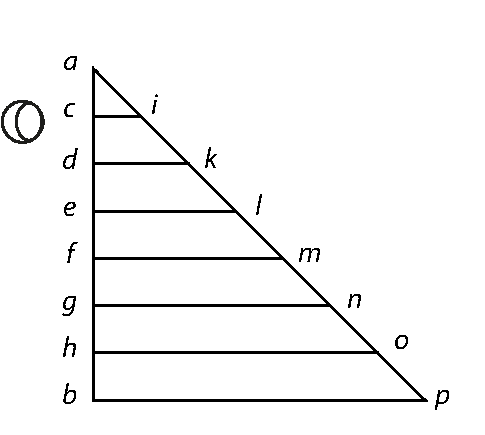
\includegraphics[trim = 0mm 3mm -5mm 0mm, clip, width=0.42\textwidth]{images/lh03705_128r-d.pdf}\\
%              \noindent \centering [\textit{Fig. 1}] 
%                        %\caption{Bildbeschreibung}
%                        \end{wrapfigure}
%Porro impetus\protect\index{Sachverzeichnis}{impetus} singuli, quovis momento accepti, comparari possunt puncto.
%\\
%\indent Ergo summa impetuum\protect\index{Sachverzeichnis}{impetus}, in quovis momento possessorum, seu impetus\protect\index{Sachverzeichnis}{impetus} integer in quovis post primum, descensus momento exhiberi potest linea.
%\\
%\indent Esto enim linea\protect\index{Sachverzeichnis}{linea tendentiae} \edtext{tendentiae a gravi descendente percurrenda}{\lemma{20f. tendentiae}\killnumber\Bfootnote{\textit{(1)}\ percursa  \textit{(2)}\ a gravi descendente percurrenda \textit{L}}} \edtext{$ab$ quae dividi intelligatur, in puncta quotlibet}{\lemma{21f. $ab$}\killnumber\Bfootnote{\textit{(1)}\ quae dividi intelligatur in puncta quotlibet \textit{(2)}\ quae et gra \textit{(3)}\ quae [...] quotlibet \textit{L}}} aequidistantia \textit{a. c. d. e. f. g. h. b}. Ponatur grave labendo pervenisse in \textit{c} manifestum est, impetum\protect\index{Sachverzeichnis}{impetus} \edtext{totum}{\lemma{24}\killnumber\Bfootnote{totum \textit{erg.} \textit{L}}} quem habet in \textit{c} esse summam tot
\pend
\newpage
\pstart \noindent impetuum\protect\index{Sachverzeichnis}{impetus} aequalium ipsi inter descendendum quaesitorum, quot sunt puncta in \textit{ac} et proinde cum impetus\protect\index{Sachverzeichnis}{impetus} singuli exhiberi possint punctis, et summae punctorum lineis, summam impetuum\protect\index{Sachverzeichnis}{impetus}, seu impetum\protect\index{Sachverzeichnis}{impetus} integrum in \textit{c} possessum, exhiberi posse linea $ci=ac$ et impetum\protect\index{Sachverzeichnis}{impetus} in \textit{d} linea $dk=ad$, et similiter erit: $ae=el$, et $af=fm$, et $ag=gn$, et $ah=ho$, et \edtext{$ab=bp$ vel potius}{\lemma{$ab=bp$}\Bfootnote{\textit{(1)}\ et impetus\protect\index{Sachverzeichnis}{impetus} \textit{(2)}\ vel potius \textit{L}\ }} cum linea descensus, cum impetibus\protect\index{Sachverzeichnis}{impetus} frustra comparetur, (heterogenea enim sunt) erit ut $ac$ ad $ad$ ita \textit{ci} ad \textit{dk} etc. Idque erit verum in omnibus punctis intermediis in \edtext{linea tendentiae}{\lemma{linea}\Bfootnote{\textit{(1)}\ descensus \textit{(2)}\ tendentiae \textit{L}\ }} assumtis, nam et lineae impetuum\protect\index{Sachverzeichnis}{impetus} omnes terminantur in recta \textit{ap} seu complent triangulum \textit{abp.} Omnes autem lineae in triangulo, basi parallelae, sunt ut altitudines.\pend 
\count\Bfootins=1200
\pstart
Si linea descensus non sit perpendicularis, seu linea tendentiae\protect\index{Sachverzeichnis}{linea tendentiae} \textit{ab} sed obliqua, ut \textit{ap} quaestio est an in linea descensus an in linea tendentiae\protect\index{Sachverzeichnis}{linea tendentiae} accipienda sint incrementa, si in \edtext{linea descensus majorem}{\lemma{linea}\Bfootnote{\textit{(1)}\ tendentiae ma \textit{(2)}\ descensus majorem \textit{L}\ }} in fine impetum\protect\index{Sachverzeichnis}{impetus} acquisivere, quae oblique descendunt, quod est absurdum. Quia inde statim sequetur motus perennis\protect\index{Sachverzeichnis}{motus perennis}, ac proinde natura nihil lucraretur. Quo posito sequitur theorema\protect\index{Sachverzeichnis}{theorema}: Vires lapsu gravium\protect\index{Sachverzeichnis}{grave} in fine acquisitas esse easdem, sive oblique, sive recta \edtext{descendant.
[128~v\textsuperscript{o}]
Porro hoc supposito}{\lemma{descendant}\Bfootnote{%
\textit{(1)} , imo etiam eodem tempore descendere [128~v\textsuperscript{o}] %
\textit{(2)} . Porro hoc supposito \textit{L}}}%
% [128~v\textsuperscript{o}]